\section{Verifiable Binomial Mechanism}
\label{sec:single_curator_hist}

This section describes how to compute counting queries verifiably with differential privacy in both the single curator and client-server MPC models. 
We consider the trusted curator model to be a special instantiation of the general MPC model where the number of provers $K=1$.
In Section \ref{sec:intuition} we describe intuitions for our protocol, and in Section \ref{sec:client-server-mpc-dp} we explain what is needed for verifiability in the MPC setting and tackle the additional challenges of verifying client inputs.
We describe how prior efforts at verifying clients fall short of the security expectations of Definition~\ref{defn:vdp_MPC}. 
Finally, in Section \ref{sec:main_protocol}, we describe a protocol that verifiably computes counting queries with DP.

Set $\mathcal{X} = \Z_q = \mathcal{Y}$, where $\Z_q$ is a prime order finite field of size $q$ over the integers. Let $X=(x_1, \dots, x_n)$ denote the client inputs and  $Q$ be the counting query $Q(X) = \sum_{i=1}^n x_i$.  Let $\share{x_i}_k$ denote the $k$'th additive secret\footnote{Although we describe our protocols with additive secret sharing, any linear secret sharing such as Shamir's secret sharing also applies to all our results.} share of a client input $x_i$. Each client splits their input into $K$ secret shares and distributes them across the provers. We will assume that $n\ll q$ and $\kappa= \lfloor \log_2 q\rfloor$ can be viewed as the security parameter. For $K \geq 1$ provers and 1 verifier, define the oracle functionality $\Mechanism_\bin$ in the ideal world as follows:
%
\begin{enumerate}
	\item{$\mathcal{M}_{\bin}$ receives public privacy parameters $\epsilon$ and $\delta$. It then computes $\noisen$ (number of coins for binomial noise) based on Lemma \ref{theorem:dp_guarantee}.}

	\item{Let $\Big(\share{x_1}_k, \dots,\share{x_n}_k\Big)$ denote the inputs on the $k$'th prover's input tape. Each prover $\Prover_k$  is expected to compute $X_k = \sum_{i=1}^n \llbracket x_i \rrbracket_k$ and sends to $\Mechanism_{\bin}$ as its input $X_k$. A corrupted prover might send an arbitrary input.} 
	
\item{$\Mechanism_{\bin}$ samples $\Delta_k \sim \texttt{Binomial}(\noisen, 1/2)$ independently for each input $X_k$ it receives. It then computes 
%
\begin{equation}
\label{eq:M_bin}
\textstyle
y =  \sum_{k=1}^K (X_k + \Delta_k)
\end{equation}
%
}
\item{$\mathcal{M}_{\bin}$ sends the tuple $(y, \Delta_k)$ as output to each prover $\Prover_k$. On receiving its output, the $\Prover_k$ sends $\texttt{CONTINUE}$ to $\Mechanism_{\bin}$. Once $\Mechanism_{\bin}$ receives the continue signal from prover $\Prover_k$ it moves on to deliver output to $\Prover_{k+1}$.}

\item{After all $K$ provers have sent $\texttt{CONTINUE}$, $\Mechanism_{\bin}$ sends $y$ as output to the verifier $\Verifier$. If a single prover fails to send the continue message and thereby exits the protocol early, the verifier and the remaining provers do not receive any output.}

\end{enumerate}

When $K=1$, i.e., the trusted curator setting, the single prover receives $n$ client inputs in plaintext, so $\share{x_i}_k = x_i$ for all $i \in [n]$. 
This is equivalent to an adversary corrupting all $K$ provers. Thus in the MPC setting with $K \geq 2$ servers, it is safe to assume at least one of them will follow the protocol.
Our goal is to be able to come up with an interactive protocol $\Pi_\bin$, 
that allows us to compute $\mathcal{M}_{\texttt{Bin}}$ verifiably as per Definition~\ref{defn:vdp_MPC}. 
Notice that in the ideal model definition above, the oracle adds $K$ independent copies of DP noise to the output, whereas 
 Lemma \ref{theorem:dp_guarantee} only calls for a single copy. 
 This is because, as we allow up to $K-1$ provers to collude with a corrupted verifier, the corrupted provers could simply not add any noise to the output. 
Ben Or \etal's completeness results  \cite{ben2019completeness} imply that $K$ independent copies of noise are \textit{necessary} to guarantee differential privacy unless the number of corruptions can be restricted to being strictly less than $\frac{K}{3}$, so each prover must independently generate enough noise to guarantee DP.
Our protocols defined below are secure against computationally bounded provers and verifiers that may deviate arbitrarily from protocol specifications and have access to auxiliary inputs.

\subsection{An Intuitive But Incomplete Protocol}
\label{sec:intuition}

Before describing the entire protocol in Section \ref{sec:main_protocol} and Figure \ref{fig:dp_interactive_proof}, we provide the reader with some intuition as to why the protocol works for a single curator and verifier. \textit{In this section, we make the unrealistic assumption that prover and verifier behave faithfully}. 
Assume all parties have joint oracle access to $\oracle_{\Morra}$ (as described in Section \ref{sec: morra}) to jointly sample unbiased bits $(b_1, \dots, b_{\noisen})$. It is easy to see that using $(\sum_{i=1}^{\noisen} b_i)$ as DP randomness results in the desired Binomial distribution defined in $\mathcal{M}_{\texttt{Bin}}$. However, the oracle output is known to both the verifier and prover; therefore, it cannot be directly used to guarantee differential privacy. 
As discussed earlier, this problem of proving that a prover faithfully sampled random bits without disclosing them lies at the heart of any verifiable DP protocol. 
Thus the protocol must combine public coins that satisfy verifiability requirements and private coins that ensure secrecy.

The protocol for verifiable DP counting proceeds in $\noisen$ identical and independent invocations (run in parallel). 
In copy $i$, the prover samples $v_i \in \bit$, which it keeps private. 
Note that a prover could sample this bit using any arbitrary bias. 
As this is the provers' private coin, the verifier has no control over how the prover generates this information. 
After the prover has sampled their private bit, the prover and verifier make one call to $\oracle_{\Morra}$ to get an unbiased coin denoted by $b_i$. 
Next, the prover locally computes  $\hat{v}_i = b_i \oplus v_i$. Here $\oplus$ refers to the boolean XOR operation. It is easy to see that $\hat{v}_i$ has the same distribution as $b_i$, but its value is known only to the parties with access to $v_i$, i.e., the prover. 
After $\noisen$ rounds, the prover computes $Q(X)$ and $Z = \sum_{i=1}^{\noisen} \hat{v}_i$ and outputs $Q(X) + Z$ where $Z$ is used as DP randomness.  By the assumption that the prover and verifier are faithful, $Z$ is distributed according to the desired distribution stated in Theorem \ref{theorem:dp_guarantee}, and its value is only known to the prover. 
To make this protocol practical, we need to resolve a few issues.

\begin{enumerate}
    \item{Although the above description requires a bitwise XOR operation to ensure the right distribution is used, we operate with arithmetic circuits in the actual protocol. 
    Thus, the provers could sample arbitrary values $v^* \in \Z_q$ such that $v^* \notin \bit$, and we need to fix how to express the XOR operation via arithmetic circuits. 
   %Secondly, it is not immediately clear what it means to do an XOR operation in arithmetic circuits with non-boolean values.
    }

    \item{Even if we could verify that the prover sampled a private bit correctly, we still need to verify that they faithfully performed the local operations discussed above.}
\end{enumerate}

Thus, if we could guarantee that each server performed its computations correctly and sampled a private value from the correct set, we would get the desired outcome of verifiable and DP counting queries.

\begin{figure}[t]
    \centering    
	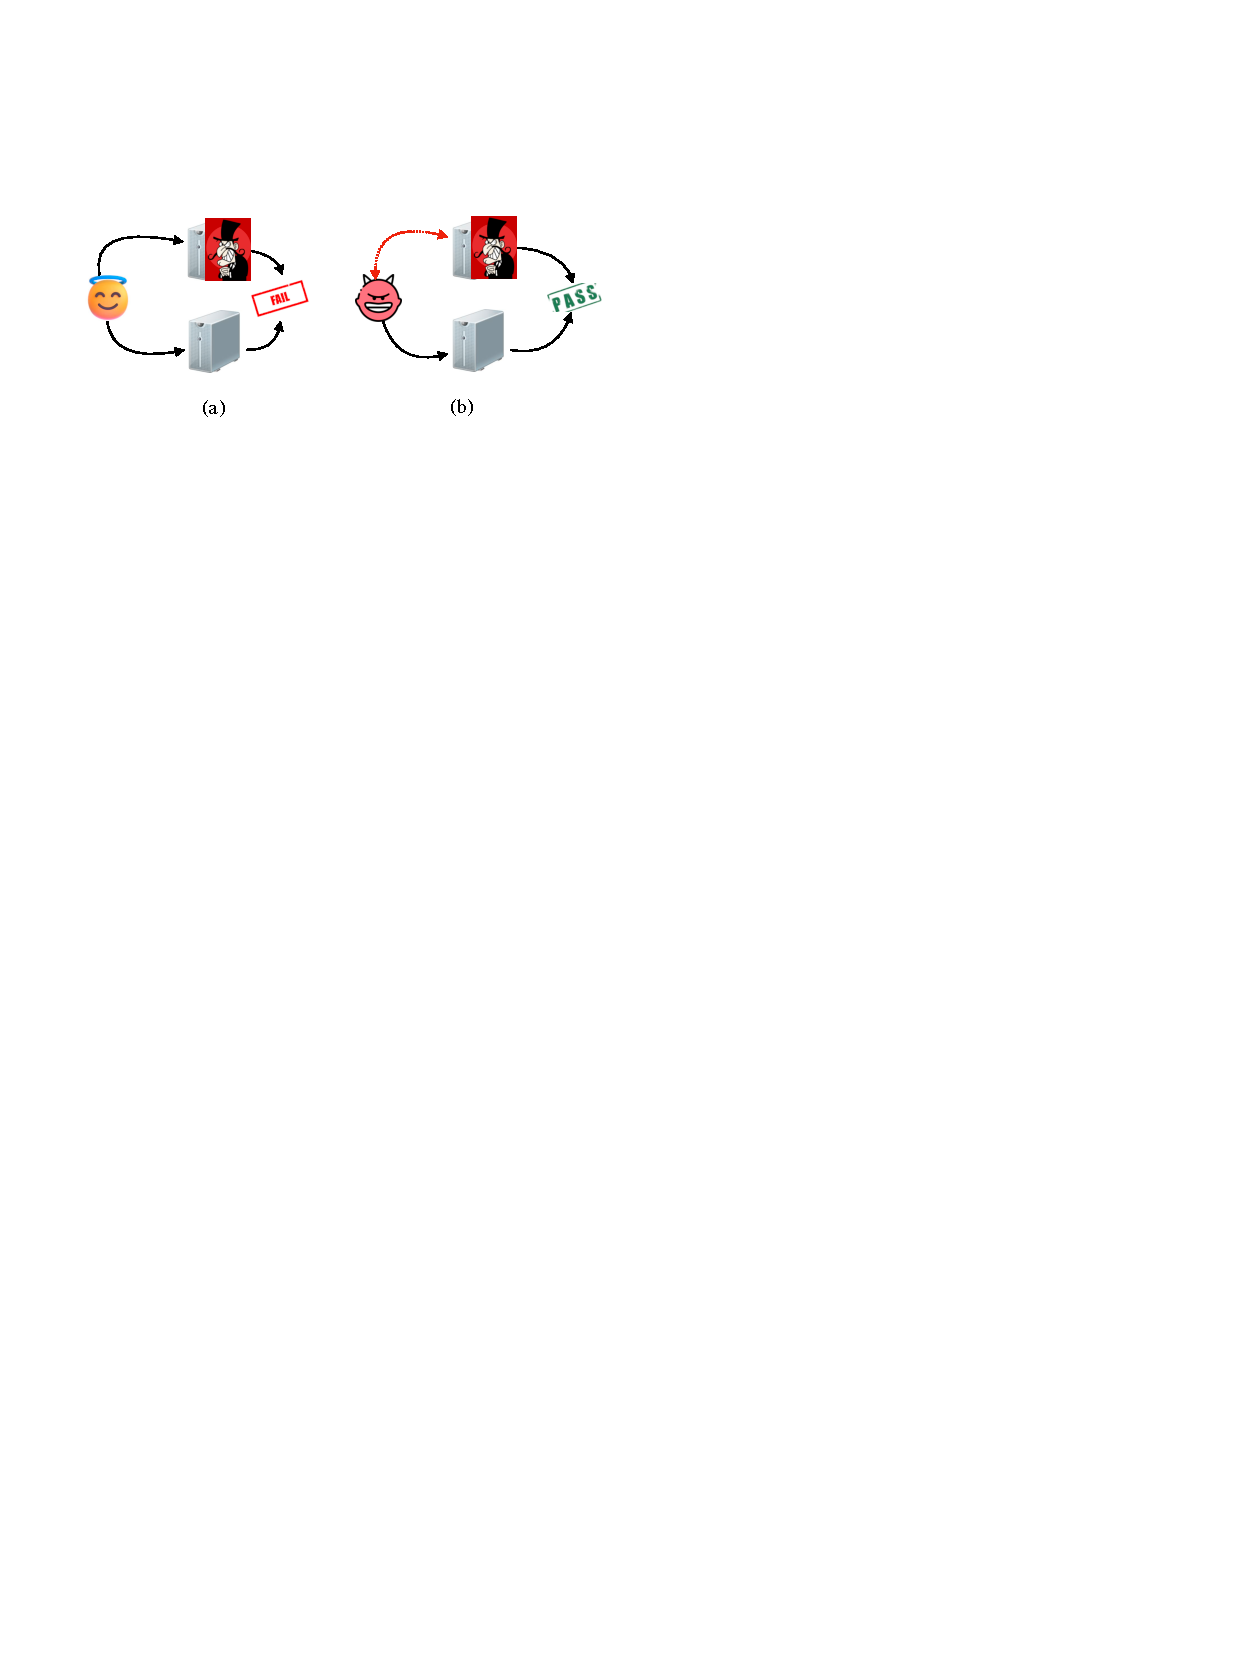
\includegraphics[scale=0.9]{pngs/attack.pdf}
	\caption{Two types of attacks that go undetected in Poplar. In (a) regardless of what the honest client sends, a corrupted server simply ignores the input and excludes the client from the protocol based on auxiliary information. In (b) a dishonest client colludes with the corrupted server by revealing secret values, so that an illegal input is included. In both cases, the honest server cannot distinguish between an honest run and a corrupted run of the protocol.}
	\label{fig:attacks}
\end{figure}

\subsection{Extending To Client-Server MPC-DP}
\label{sec:client-server-mpc-dp}

To compute DP histograms verifiably in the client-server MPC-DP setting, we use the same computational model used for PRIO \cite{corrigan-gibbs_prio_2017} and Poplar \cite{boneh_lightweight_2022}. Prio is deployed at scale by Mozilla \footnote{\url{https://blog.mozilla.org/security/2019/06/06/next-steps-in-privacy-preserving-telemetry-with-prio/}}.
As discussed earlier, in this setting $n$ clients secret share their inputs $x_i \in L$ amongst $K \geq 2$ provers, where $L \subseteq \mathcal{X}$ defines the language of legal inputs to the protocol. 
For computing $M$-bin histograms over $n$ inputs, $L$ is the set of all one-hot encoded vectors of size $M$. 
For the core problem of a single-dimensional counting query, we have $M=1$ and $L=\bit$.  
Since the inputs on the prover's tapes reveal no information about a client's input, for the protocol to be useful the provers must first verify in zero knowledge that $x_i \in L$ before using such inputs to compute aggregate statistics. 
This additional step of verifying a client is not required in the trusted curator model, as the prover decides what inputs should be included in the computation and can see them in plaintext.

\paragraph{Verifying Clients in MPC-DP}
\label{sec:client_verification}

Poplar and PRIO use efficient sketching techniques from \cite{boyle_function_2016} to validate a client's input in zero knowledge \textit{without} relying on any public key cryptography. Thus, as long as at least one out of $K$ provers does not reveal the inputs it received, even an unbounded adversary corrupting the remaining provers cannot ascertain any information about an honest client's input. While such a system protects an honest client's privacy from an unbounded adversary, it is not verifiable as per Definition \ref{defn:vdp_MPC}. 
Specifically, for the techniques used in PRIO and Poplar, a single corrupted prover could tamper with its inputs and exclude an honest client from the protocol by forcing them to fail the verification test. 
Alternatively, a corrupt client could collude with a prover to include arbitrary inputs, jeopardising the correctness of the output. 
Figure\footnote{Content from J.J. at the English-language Wikipedia, licensed under \href{https://creativecommons.org/licenses/by-sa/3.0/deed.en}{CC BY-SA 3.0}.}~\ref{fig:attacks} summarises these attacks on Poplar and PRIO\footnote{Concretely, referring to  notation from \cite[Appendix C]{boneh_lightweight_2022}, in scenario (b), the dishonest client reveals the values $\kappa$ and $[v]_0$ to the server. This allows the server to set $z_1 = -z_0, z_1^* = -z_0^*$ and $z_1^{**} = -z_0^{**}$, thereby 
 admitting an illegal input into the protocol.}. By our definitions of verifiability, the protocol's output \textit{must} be a function of the inputs provided by honest clients only. 
 Thus the protocol described in Section \ref{sec:main_protocol} provides the following additional guarantees:

\begin{enumerate}
	\item{\textbf{Guaranteed Inclusion Of Honest Clients}: If a client submits shares of an input $x \in L$, then the final output of the protocol is guaranteed to use this input untampered. Thus an honest client is assured that, as long as a single prover follows the protocol specifications, no one learns any information about their private input and their input is correctly used to compute the final output. }
	\item{\textbf{Guaranteed Exclusion Of Corrupt Clients}: A corrupted client, even one that has control over any proper subset of the $K$ provers, cannot include an invalid input to the protocol. Thus if $x \notin L$, $x$ is discarded by our protocol with overwhelming probability.}
\end{enumerate}

It is important to note that as we operate under stricter notions of privacy and correctness, our results require the use of public-key cryptography and security holds only against computationally bounded adversaries.  Furthermore, we show in Section \ref{sec:separation} that it is impossible to satisfy verifiable DP and provide information theoretic guarantees.

\begin{figure*}[h]
    \centering
\begin{pchstack}[boxed]  % default  
    \pseudocode[linenumbering , skipfirstln]{%
    \textbf{ Verifier}(\Verifier) \< \< \textbf{Prover}(\Prover_k) \\[][\hline]
    \pp \samples \texttt{Setup}(1^\SecurityParam) \< \text{Generate public parameters} \<   \pp \samples \texttt{Setup}(1^\SecurityParam) \\
	\Bigg\{  \Big\{ c_{i,k}  \Big\}_{k \in [K]} \Bigg\}_{i \in [n]} \< 
 \text{Client inputs }  \<  \Big\{ \share{x_i}_k, r_{i,k} \Big\}_{i \in [n]}, 	\Bigg\{  \Big\{ c_{i,k}  \Big\}_{k \in [K]} \Bigg\}_{i \in [n]}\\
     \forall i \in [n] \text{ Send } c_{i} = \prod_{k=1}^K c_{i,k}  \<  \oracle_{\OR} \<   \forall i \in [n] \text{ Send } c_{i} = \prod_{k=1}^K c_{i,k}\\
\text{For any } i \in [n] \text{ if }\oracle_{\OR}(c_{i}) \neq 1\<\text{Exclude } (\share{x_i}_k, r_{i,k}) \text{ from the protocol} \<  \\
    (c'_{1,k}, \dots, c'_{{\noisen},k})\< \sendmessageleft*{c'_{j,k} = \Com\Big( v_{j,k}, s_{v_{j,k}}\Big)} \< \forall j \in [\noisen] \text{ Samples and commits } v_{j,k} \in \bit \text{}\\    
    \forall j \in [\noisen]\text{ Send } c'_{j,k} \< 
\oracle_{\OR}  \<  \forall j \in [\noisen] \text{ Send openings} (v_{j,k}, s_{j,k})\\    
    \forall j \in [\noisen]\text{ Check } \oracle_{\OR}(c'_{j,k}) = 1\<\<  \\
    \forall j \in [\noisen]\text{ Send empty string } \lambda_j \< 
\oracle_{\Morra} \< \forall j \in [\noisen]\text{ Send empty string } \lambda_j\\
    \text{ Receive } (b_{1,k}, \dots, b_{\noisen,k}) \< 
 \forall j \in [\noisen] \text{ }b_{j,k} = \oracle_{\Morra}(\lambda_j) \text{ } \< \text{ Receive } (b_{1,k}, \dots, b_{\noisen,k})\\  \< \< \forall j \in [\noisen] \text{ Update }v_{j,k} , s_{j,k}  \text{ to get }  \hat{v}_{j, k}, \hat{s}_{j, k} \\
 \<\<\text{ based on }  b_{j,k}\\ 
  \<  \< y_k = \sum_{i=1}^n \share{x_i}_k + \sum_{j=1}^{\noisen} \hat{v}_{j,k} \text{ and } \\
  \< \sendmessageleft*{(y_k, z_{k})} \< z_{k} = \Big(\sum_{i=1}^{n}r_{i,k}+ \sum_{j=1}^{\noisen} \hat{s}_{j,k}\Big) \\  
    \text{Compute } \hat{c}'_{j,k} \text{ using } b_{j,k}  \text{ for all } j \in [b_{\noisen}]\< \<  \\    
  \text{Check } \Big( \prod_{i=1}^{n} c_{i,k} \times \prod_{j=1}^{\noisen} \hat{c}'_{j,k}\Big) \< \< \\
  \qquad = \Com(y_k, z_{k})\< \<
}
\end{pchstack}    
\caption{The figure above describes the interaction between a single prover and verifier in $\Pi_{\bin}$. In the single trusted curator model $K=1$ we have $x_i = \share{x_i}_k$ where the prover can see client inputs in plaintext. In the MPC setting, each prover $\Prover_k$ follows the exact same protocol on their respective inputs specified in Line 2. Thus at the end of the protocol, each prover $\Prover_k$ outputs the tuple $y_k, z_{k}$. A verifier aggregates the output from each prover to publish verifiable DP statistics. }
    \label{fig:dp_interactive_proof}
\end{figure*}


\subsection{Main Protocol Description}
\label{sec:main_protocol}

The protocol $\Pi_{\bin}$ described in Figure \ref{fig:dp_interactive_proof} provides a compact standalone description of the interaction between $K$ provers and the verifier for computing $\Mechanism_\bin$. 
We assume that both the provers and the verifier have access to oracles $\oracle_{\Morra}$ and  $\oracle_{\OR}$ as defined in Section \ref{sec: commitments}. 
In the real world, $\oracle_{\Morra}$ is replaced with $\Pi_{\Morra}$ (see Algorithm \ref{alg: morra}) and $\oracle_{\OR}$ is replaced by Cramer \etal's $\Sigma$-OR proof \cite{cramer1994proofs} (see Appendix \ref{app:sigma_open} for an example implementation) which securely compute the oracle functionalities in the presence of adversaries that may deviate from protocol specifications. Thus, we define our protocol in the hybrid world, and by the sequential composition theorem\footnote{Though we use sequential composition, both protocols $\Pi_{\Morra}$ and $\Pi_{\OR}$ can be composed in parallel.} \cite{goldreich_foundations_2007}, the security properties of the protocol are preserved. 
Next, we describe the protocol in detail with line references to Figure \ref{fig:dp_interactive_proof}:

\begin{enumerate}
    \item[Line 1:]{ In the first step, the prover(s) and verifier agree upon the public parameters for the protocol. The public parameters include a description of $\mathcal{C}_\pp = \G_q, \mathcal{M}_\pp = \mathcal{X} = \mathcal{Y} = \Z_q, \RandomnessSpace_\pp= \Z_q$ and a description of $\mathcal{M}_\texttt{bin}$ as defined in equation \eqref{eq:M_bin}. 
    The group $\G_q$ satisfies the requirements of the homomorphic commitment scheme defined in Section \ref{defn:hom_coms} and we assume that the discrete log problem is hard to solve in $\G_q$.}

\item[Line 2:]{ For each client $i \in [n]$, let $\share{x_i}_k$ denote the $k$'th share of their input $x_i \in L$. 
Define $c_{i,k} = \Com\Big(\share{x_i}_k,  r_{i,k}\Big)$ as the commitment to the $k$'th share of $x_i$. 
The client sends to each prover $\Prover_k$ the tuple $(\share{x_i}_k,  r_{i,k})$ and broadcasts 
the commitments to each of the shares $\Big( c_{i,1}, \dots, c_{i,K} \Big)$ to a public bulletin board that is observable to all parties.}

\item[Line 3-4:]{Similar to PRIO and Poplar, we use $L=\bit$, and thus verifier and the client use the oracle $\oracle_{\OR}$ to check if the client's input is indeed a commitment to a bit. 
For input $x_i$, the verifier (and provers) sends to  $\oracle_{\OR}$ the derived commitment $c_{i} = \prod_{k=1}^K c_{i,k}$ and the client sends the openings $\Big(x_i, \sum_{k=1}^K r_{i,k}\Big)$. 
The oracle responds with $\oracle_{\OR}(c_{i}) = 1$ if $x_i \in \bit$ and $c_i$ is a commitment to $x_i$.
In the real world, we replace $\oracle_{\OR}$ with a $\Sigma$-OR protocol \footnote{In the interactive setting, the verifier, the provers, and the client jointly sample a public challenge by playing Morra. As long a single party is honest, the challenge is guaranteed to be selected uniformly at random. Alternatively, in the ROM model, the client sends to a public bulletin board a non-interactive $\Sigma$-proof using the Fiat-Shamir transform.}. This step resolves the issues presented in Figure~\ref{fig:attacks}, as an honest client cannot be excluded nor can a corrupt client input be included. From here on, the protocol only uses inputs from validated clients.}
%
\item[Line 5:]{$\Prover_k$ samples $(v_{1,k}, \dots, v_{\noisen,k})$ where $v_{j,k} \in \bit$ (private random bit) and sends to the verifier commitments to $v_{j,k}$ for $j \in [\noisen]$. 
    Let $c'_{j,k} = \Com(v_{j,k}, s_{j,k})$ denote the commitment to $v_{j,k}$ with randomness $s_{j,k}$. To enforce consistency in notation and improve readability, we always use $c$ to denote commitments to client inputs and $c'$ to denote commitments to the prover's private inputs. Similarly, we will always use $r$ and $s$ to denote the randomness used for client input and prover bit commitments, respectively.}    
%
\item[Line 6-7:] {The verifier uses $\oracle_{\OR}$ to check if the messages sent by the prover were indeed commitments to 0 or 1 (similar to verifying client inputs). 
This step is essential for the Boolean to arithmetic conversion, as the linearisation of the XOR operation is only valid for values $v \in \bit$ (see completeness property of Theorem~\ref{theorem:verifiable_dp_feasible}).}

\item[Line 8-9:]{If for any $i \in \noisen$, $\oracle_{\OR} = 0$, the verifier aborts the protocol and broadcasts that $\Prover_k$ cheated. Otherwise, once all commitments are verified, the prover and verifier jointly invoke $\oracle_{\Morra}$ to get $\noisen$ \textit{public} unbiased bits $(b_{1,k}, \dots, b_{\noisen,k})$.}

\item[Line 10-11:]{For all $i \in [\noisen]$, based on the value of $b_{j,k}$, the prover sets $\hat{v}_{j,k}$ and $\hat{s}_{j,k}$ as follows
    %
    \[   
    \hat{v}_{j,k} = 
         \begin{cases}
        1 - v_{j,k} & \text{if } b_{j,k}=1\\
        v_{j,k}& \text{otherwise.} \\ 
     \end{cases}
\]

    \[   
    \hat{s}_{j,k} = 
         \begin{cases}
        1 - s_{j,k} & \text{if } b_{j,k}=1\\
        s_{j,k}& \text{otherwise.} \\ 
     \end{cases}
\]

As long as $v_{j,k} \in \bit$, the above set of equations is equivalent to setting $\hat{v}_{j,k} = v_{j,k} \oplus b_{j,k}$. An important feature of this step is that, conditioned on $b_{j,k}$, the operations described above are linear. Line 11 describes why this is critical for correctness to hold.
}

    \item[Line 12-13:]{The prover sends $(y_k, z_{k})$ to the verifier:
    \begin{equation}
    y_k = \Big(\sum_{i=1}^n  \share{x_i}_k + \sum_{j=1}^{\noisen} \hat{v}_{j,k} \Big) 
    \end{equation}    
    \begin{equation}
    z_{k} = \Big(\sum_{i=1}^n r_{i,k} + \sum_{j=1}^{\noisen} \hat{s}_{j,k}\Big)     
    \end{equation}
    
    where $(y_k, z_{k})$ is the output for prover $\Prover_k$.
    }

    \item[Line 14:]{Using the common public randomness $\{ b_{j,k} \}_{j \in [\noisen]}$ generated by $\oracle_{\Morra}$, the verifier updates their view of received commitments as follows:

      \[   
\hat{c}'_{j, k} = 
     \begin{cases}
       \Com(1, 1) \times {c'}_{j, k}^{-1} & \text{ if } b_{j, k}=1\\
       c'_{j, k}&\quad\text{otherwise.} \\ 
     \end{cases}
\]
    Note that $\Prover_k$ never opens $\hat{c}^\prime_{j, k}$, and thus $\Verifier$ never sees $\hat{v}_{j, k}$ in plaintext. By the hiding property of commitments, an efficient verifier learns nothing about the prover's private values from these messages. However, as the update conditioned on $b_{j, k}$ is linear and $b_{j, k}$ is public, $\Verifier$ can still compute a commitment to $1 - v_{j, k}$ without ever knowing $v_{j, k}$. As a direct consequence, as discussed in the soundness claim, the prover cannot deviate from its prescribed linear operation, as the verifier can check it.
    As we will show later, this step guarantees correctness, soundness and security. 
    }
    \item[Line 15-16:]{Finally, the  verifier checks 
    \begin{equation}
    \label{eq:vfr_check}
     \prod_{i=1}^{n} c_{i,k} \times \prod_{j=1}^{\noisen} \hat{c}'_{j, k} = \Com(y_k, z_k)   
    \end{equation}        
    }    
\end{enumerate}

From these outputs, we can derive the desired result: we treat the $y_k$'s as shares, and calculate $y = \sum_{k=1}^{K} y_k$ as the noisy sum.  
We next show that this protocol achieves our desired properties. 
\begin{thm}
\label{theorem:verifiable_dp_feasible} 
Let $X=(x_1, \dots, x_n)$ be the client input. Let $\Mechanism_\bin$ and $\oracle = (\oracle_{\Morra}, \oracle_{\OR})$ be as defined above.  $\Pi_{\bin}$ is a verifiably differentially private argument with perfect completeness, negligible soundness and is computational zero knowledge.

%%then the following is true
%%
%%    \item{\textbf{Completeness:} For every $X \in \mathcal{X}^n$ 
%%%    
%%     \[ \Pr\left[ \texttt{out}(\Vfr, \vec{\Pv}) = 0 : \begin{array}{c} \pp \leftarrow \texttt{Setup}^\oracle(1^\kappa) \\
%%     \Pv_k^\oracle \leftarrow \share{X}_k, \bvec{r}_{\Pv_k}, \pp \\
%%     \Vfr^\oracle \leftarrow z, \bvec{r}_v, \pp \\
%%y \leftarrow \Pi_\bin^\oracle(\vec{\Pv}, \Vfr)
%%    \end{array} \right]
%%  = 0  \] 
%%  
%%  where $\share{X}_k = (\share{x_1}_k, \dots, \share{x_n}_k)$ and $\bvec{r}_{\Pv_k}$ denotes $\Pv_k$'s private randomness.
%%  }
%%
%%\item{\textbf{Computational Soundness:} For every $X \in \mathcal{X}^n$ and any subset $I \subseteq [K]$, let $\vec{\Pv^*}$ denote the collection of provers, indexed by $I$, that have been corrupted by an adversary $\AdvA$, such that the final output $y \neq \Mechanism_\bin(X, Q)$. Let $\vec{\Pv}$ denote the collection of honest provers not indexed by $I$. Let $z$ denote the auxiliary input available to $\AdvA$ and $\mu$ be its advantage in the discrete log game (Definition \ref{defn:discrete_log}) 
%%
%%  \[ \Pr\left[ \texttt{out}(\Vfr, \vec{\Pv^*}, \vec{\Pv}) = 1 : \begin{array}{c} \pp \leftarrow \texttt{Setup}^\oracle(1^\kappa) \\
%%     \Pv_k^\oracle \leftarrow \llbracket X \rrbracket_k, \bvec{r}_{\Pv_k}, \pp \\
%%     \Vfr^\oracle \leftarrow z, \bvec{r}_v, \pp \\
%%y \leftarrow \Pi_\bin^\oracle\Big((\vec{\Pv}, \vec{\Pv^*}), \Vfr\Big)
%%    \end{array} \right]
%%  \leq \mu(\kappa)  \] 
%%  
%%Note that as $I \subseteq [K]$, soundness, as defined above, covers both the MPC and the trusted curator setting.
%%}
%%     
%%    \item{\textbf{Computational zero knowledge}: 
%%Let $\vec{\Pv^*}$ denote the collection of provers, indexed by $I \subset [K]$, that have been corrupted by a corrupt verifier $\Vfr^*$. There exists a PPT Simulator $\Sim_{(\Vfr^*, I)}$ such that for all $y = \mathcal{M}(X, Q)$
%%    \begin{align*}
%%    \texttt{View}\Bigg[\Pi\Big((\vec{\Pv}, \vec{\Pv^*}), \Vfr^*, \pp\Big)\Bigg] &\stackrel{c}{\equiv} \Sim_{(\Vfr^*, I)}(y, \bvec{r}_v, z, \pp)        
%%    \end{align*}
%%
%%    Where $z \in \bit^{\texttt{poly}(\kappa)}$ and $\bvec{r}_v \in \bit^{\texttt{poly}(\kappa)}$ represents auxiliary input and randomness available to all the corrupted parties.
%%    }
%
%
\end{thm}

\begin{proof}
\

\paragraph{\textbf{Completeness:}}
By the definition of $\oracle_{\Morra}$, $(b_{1,k}, \dots, b_{\noisen,k})$ are all unbiased bits. 
As per $\Pi_{\bin}$, when $b_{j,k}=1$, $\hat{v}_{j,k}=1-v_{j,k}$ and when $b_{j,k}=0$, $\hat{v}_{j,k} = v_{j,k}$. 
We know that an honest prover is guaranteed to have sampled a private value $v_{j,k} \in \bit$ for all $j \in [\noisen]$. 
Thus the case-wise arithmetic operation described above is equivalent to setting $\hat{v}_{j,k} = v_{j,k} \oplus b_{j,k}$. 
This implies that for each server $\hat{v}_{j,k} \xleftarrow{R} \bit$ and $\sum_{j=1}^{\noisen} \hat{v}_{j,k} \sim \texttt{Binomial}(\noisen, 1/2)$. 
The output of each honest prover is thus $y_k = \texttt{Binomial}(\noisen, 1/2) + \sum_{i=1}^n \share{x_i}_k$. 
By linearity of secret-sharing, $\sum_{k \in [K]} y_k = \mathcal{M}_{\bin}(X, Q)$ where  $\mathcal{M}_{\bin}$ is defined in equation \eqref{eq:M_bin}. 

\paragraph{\textbf{Soundess}}
Beyond exiting the protocol early (which is trivially detected), an adversary $\AdvA$ controlling a collection of dishonest provers could force a prover to cheat by doing at least one of the following:

\begin{enumerate}

    \item{ (Cheat at Line 4): For any $j \in [\noisen]$, $c'_{j,k}$ is not a commitment to a bit. As the verifier has access to oracle $\oracle_{\OR}$, it would detect this immediately. Thus we can be guaranteed that $c'_{j,k}$ are commitments to 1 or 0.}

    \item{(Cheat at Line 7): The prover could sample improper public randomness. 
    However, this is impossible as the verifier and prover jointly use $\oracle_{\Morra}$ to generate randomness.}
    
    \item{(Cheat at Line 13): Output messages $(y_k^\prime \neq y_k$, $z_{k}^\prime \neq z_{k})$. 
    If the verifier check from (Line 15) fails then the verifier knows $\Prover_k^*$ cheated. If 
      $\Com(y_k, z_{k}) = \prod_{i=1}^{n} c_{i, k}\times \prod_{j=1}^{\noisen} \hat{c}'_{j,k} = \Com(y_k^\prime, z_{k}^\prime)$, then $\AdvA$ has broken the binding property of the commitment scheme. As $\AdvA$ has negligible success in winning the discrete log game, it has a negligible chance at breaking the commitment scheme. 
    }
\end{enumerate}

These are the only places where the $\ChProver$ sends a message to the $\Verifier$, and thus we have our result.

\paragraph{\textbf{Zero Knowledge}}

To prove zero knowledge, we need to define the commitment scheme we are using explicitly. We use Pedersen Commitments, which are defined as follows 
\begin{equation}
\label{eq:ped_com}
    \Com(x, r) = g^xh^{r}
\end{equation}
\noindent
where $\RandomnessSpace_\pp = \mathcal{M}_\pp= \Z_q$ and $\mathcal{C}_\pp = \G_q$ is an abelian group where the discrete log problem is hard. To enhance readability, we will prove security for  $K=2$ provers and one verifier, but the result trivially generalises to $K \geq 2$ provers. To avoid confusion between the MPC and single curator setting, we defer the simpler security proof for single curators to Appendix \ref{app:single_curator_sec_proof}. 
Without loss of generality, assume that the verifier $\ChProver$ and $\Prover_1$ have been corrupted by a PPT adversary $\AdvA$ and that $\Prover_2$ is honest. 
$\Simulator$ receives on its input tape the inputs for $\Prover_1$ and $\Verifier^*$. The ideal oracle functionality $\Mechanism_\bin$ is defined as before. Let $\Simulator$ denote shorthand for $\Simulator_{\ChVerifier, \Prover_1}$.  We construct the simulator as follows:

\begin{enumerate}
    
    \item{$\Simulator$ receives the public messages $\Bigg\{  \Big\{ c_{i,k}  \Big\}_{k \in [K]} \Bigg\}_{i \in [n]}$ and sets $c_{i} = \prod_{k=1}^K c_{i,k}$.}

    \item{$\Simulator$ internally invokes $\Prover_1$ to receive inputs $X_1$. If $\Prover_1$ was honest then $X_1 = \sum_{i=1}^n \llbracket x_i \rrbracket_1$. Of course, we have no control over $\AdvA$, and $X_1$ could be any arbitrary value. The definition of security requires that we prove security using the actual inputs used by the real-world adversary $\AdvA$ and not the ones it was handed to at the start of the protocol.}

    \item{$\Simulator$ invokes $\Mechanism_\bin$ with input $X_1$ and receives $(y, \Delta_1)$ as defined in equation \eqref{eq:M_bin}. Note $\Simulator$ never has access to the honest party's input $X_2$ nor the randomness $\Delta_2$ used by $\Prover_2$ in the real protocol. It must simulate the messages and output of the real protocol from just its input and the output it receives from the ideal model.}

    \item{$\Simulator$ sets $y_1= X_1 + \Delta_1$ and computes $y_2 = y - y_1$, which by the definition of $\Mechanism_\bin$, is equal to $(X_2 + \Delta_2)$.}

    \item{$\Simulator$ samples $z_2 \samples \RandomnessSpace_\pp$ and sets $c_{2} = \Com(y_2, z_{2})$.}

    \item{$\Simulator$ samples $c'_{2,2}, \dots, c'_{{\noisen},2}$ such that $c'_{j,2} = \Com(1, s_{j,2})$ where $s_{j,2} \samples \RandomnessSpace_\pp$. 
     It sets $c'_{1,2} = g^1a_2$ where $a_2 = c_{2} \times  \Big( \prod_{j=2}^{\noisen} \hat{c}'_{j,2}\Big)^{-1} \times \Big( \prod_{i=1}^{n} c_{i,2}\Big)^{-1} \times g^{-1}$. 
     Notice that $\Simulator$ is actually unable to open $c'_{1,2}$ but is never required to do so, as opening a commitment to a private value violates DP. The only information $\AdvA$ can check is if $c'_{1,2}$ is a commitment to a bit, which it is. Thus the simulator artificially constructs a set of commitments that align with the real-world protocol, without having the slightest idea what the randomness used by $\Prover_2$ actually was. It is able to do so due to the hiding property of the commitment scheme.}
    
     \item{$\Simulator$ sends over $\{c_{j,2}\}_{j \in [\noisen]}$ to $\AdvA$ pretending to be the honest prover (Line 4 of Figure \ref{fig:dp_interactive_proof}).}
	    
    \item{$\Simulator$ pretends to be the prover and jointly invokes $\oracle_{\Morra}$ with $\AdvA$ to sample $\noisen$ unbiased public bits $(b_{1,2}, \dots, b_{\noisen,2})$.}
    
    \item{$\Simulator$ sends $y_2$ and $z_{2}$ to $\AdvA$ and outputs whatever $\AdvA$ outputs.}
    \end{enumerate}
\end{proof}
%
\subsection{Public Verifiability and Randomness}

Notice that the verifier does not contribute a private input to the protocol, and its messages contain no private information either. 
Furthermore, any party (the clients or the prover) may view the messages sent and received by the verifier.
The verifier's role is primarily to generate unbiased public randomness (independent of the prover's messages), which is used to ensure soundness. 
It samples a challenge for the $\Sigma$-OR proof to verify that the prover's private values are well formed.
Additionally, it participates in Morra, to generate unbiased public coins to enforce the prover's DP noise is sampled from the correct distribution. 
In the computational complexity literature, such a verifier is called a public coin verifier \footnote{\url{https://en.wikipedia.org/wiki/Interactive_proof_system}}. 
If there was another way to sample unbiased and reliable randomness without the verifier, anyone accessing the message transcript could verify if soundness holds.  Consider the Random Oracle Model (ROM), where the verifier's randomness generation (Morra) is replaced by applying a random oracle on the prover and client messages.
Further, consider that all messages from the prover(s) are sent to a public bulletin board along with the client's input commitments and timestamps, with the slight modification that the prover sends commitments and non-interactive proofs of validity \textit{before} the clients send messages to the board. 
The order matters as this prevents the prover from adaptively selecting private values based on the clients' messages, thereby biasing the output of applying a ROM on the board's contents. This way, the prover's messages are guaranteed to be independent of the honest client's messages.
Now, any party (including the clients or even one that did not participate in the protocol) can verify that the randomness is correctly generated (using the oracle on the bulletin board messages) and then perform the checks assigned to the verifier to ensure soundness holds. 
There is no longer a need for parties to play Morra to generate reliable randomness.
Thus, we do not need an explicit verifier.
Such a protocol, where the correctness of the output can be verified by a non-participating entity, even when all participants responsible for computing the output are corrupted, is said to be publicly or universally verifiable (Definition~1 of \cite{baum2014publicly}). Public verifiability is a critical property for protocols such as E-voting \cite{harrison2022vericondor}, where one cannot trust a single verifier or a small group to help compute the output reliably. 
Of course, the ROM model is a theoretical construct. In the real world, we do not have a provable instantiation of a random oracle. 
Thus the protocol described above is not verifiable unless we assume at least one party (the verifier or one of the provers) is semi-honest. 
This semi-honest participant ensures that the public randomness is sampled reliably.
So the question beckons, can we upgrade interactive proofs of differential privacy from verifiability to public verifiability in the plain model? Next we show that public verifiability (as defined in Definition~1 of \cite{baum2014publicly}) is impossible for interactive proofs for differential privacy if all participants are corrupted. Thus, the trust assumptions in our protocol above are the best we can hope for. 

Unlike deterministic E-voting protocols, the outputs of a differentially private mechanism are, by definition, random. 
Furthermore, the output is a function of the client's inputs and the prover's private randomness. In end-to-end auditable voting \cite{adida2008helios, harrison2022vericondor} or publicly verifiable MPC \cite{baum2014publicly}, the output of the protocol is a deterministic function of the client inputs only. 
Correctness is measured with respect to the output of an ideal functionality computing the desired function over these inputs. 
For DP mechanisms, the prover is responsible for providing a private but random input, which is used along with client inputs to compute a DP statistic. 
Thus in this setting, the prover has more agency to affect the output than the computing parties in an universally auditable MPC.
The core problem for verifiable differential privacy lies in verifying that the final DP randomness comes from the correct distribution (an unbiased binomial distribution in our case) without learning anything about the prover's private random sample. 
Thus to verify a claim about a DP statistic, at the very least, we need a source for public and verifiable randomness.
This is to say that the DP randomness must be computed as a joint function of the prover's private randomness and reliable public randomness to enforce both secrecy and verifiability. 
Without reliable public randomness, we cannot make a meaningful claim about the final output distribution.
Thus a source of verifiable public randomness is necessary for verifiable DP.  Such sources of public randomness are often called random beacons in the blockchain literature \footnote{\url{https://a16zcrypto.com/content/article/public-randomness-and-randomness-beacons/}.}.
In the plain model (without a common random string (CRS) or a random oracle), we either need a trusted party to generate public randomness or require that the public randomness be computed using MPC among the participants.
In the protocol above, we generate public randomness using Morra, one possible MPC instantiation of a random beacon (based on the classic commit and reveal approach). 
MPCs based on Verifiable Delay Functions (VDFs) can also generate public randomness with guaranteed output delivery \cite{boneh2018verifiable}.
 Both Morra and VDFs require that at least one participant be semi-honest. In general, if all participants of the randomness-generating MPC are corrupted, then we cannot guarantee reliable public randomness. 
Thus in the plain model, we cannot guarantee public verifiability if all parties are corrupted, giving us the following corollary. 

\begin{corollary}
\label{thm:impossible_public_verif}
Provided that there is at least one honest participant or a reliable source of public randomness (random beacon), the transcript of $\Pi_\bin$ can be efficiently verified by any party (even one that did not participate in the protocol). Absent this, it is impossible to provide universal verifiability in the plain model.
\end{corollary}
